\documentclass[11pt]{article}
\usepackage[margin=1in]{geometry}
\usepackage{booktabs}
\usepackage{multirow}
\usepackage{graphicx}
\usepackage{url}
\usepackage{xcolor}
\usepackage{hyperref}
\usepackage{natbib}

\newcommand{\todo}[1]{\textcolor{red}{[TODO: #1]}}

\title{FinIF: Can Large Language Models Follow Instructions in Financial Tasks?}
\author{Anonymous ACL submission}
\date{}

\begin{document}
\maketitle

\begin{abstract}
Financial LLM applications rarely ask for free-form answers alone: they require grounded work products that obey explicit delivery constraints, such as evidence placement, quantitative lineage, approval boundaries, missing-information handling, and output format. Existing instruction-following benchmarks emphasize general constraints, while financial benchmarks mainly measure knowledge, reasoning, or answer quality. We introduce FinIF, a finance instruction-following benchmark suite consisting of FinIF-Test and FinIF-Train. FinIF-Test is a 300-item hard benchmark covering 38 financial workflow tasks and 3,134 instruction-following constraints. FinIF-Train contains 1,064 workflow-grounded examples with 7,851 annotated constraints for training and data expansion. FinIF is built by a scalable pipeline that constructs context packs, workflow-specific queries, explicit constraints, and evaluation protocols. Its evaluator combines deterministic rule checkers with item-batched LLM judging, reporting both constraint-level compliance and strict item-level pass rate. Experiments show that strong models can satisfy most individual constraints while still failing many complete financial work products: GPT-5.5 reaches 93.30\% constraint-level compliance but only 58.67\% strict item-level pass rate, while GPT-5 reaches 91.35\% and 47.33\%, respectively. Error analysis shows persistent failures in evidence placement, quantitative verification, and decision-boundary reasoning. Code and data will be released at \href{xxx}{GitHub}.
\end{abstract}

\section{Introduction}

Large language models (LLMs) are increasingly used for financial analysis, compliance review, investment due diligence, reporting, and operations support. These tasks are not simple open-domain questions. A financial user usually provides explicit source materials, asks for a well-defined work product, and states delivery requirements that control how the answer should be used downstream. For example, a model may need to prepare a credit memo, suitability review, reconciliation exception report, or compliance escalation note while citing active source labels, separating facts from assumptions, showing calculation inputs, preserving exact thresholds, and avoiding unsupported approval or legal conclusions.

This setting exposes a gap in current evaluation. A model can be financially plausible yet operationally unusable if it ignores delivery constraints. A response that reaches the right high-level recommendation may still fail because citations appear only at the end, a calculation lacks source inputs, a risk label is softened, or an approval boundary is omitted. In high-stakes workflows, such failures are not cosmetic. They break audit trails, weaken reviewability, and can create compliance risk.

However, existing benchmarks only partially cover this problem. General instruction-following benchmarks such as IFEval and FollowBench evaluate whether models obey verifiable or fine-grained constraints, but their tasks are not grounded in financial work products. Financial benchmarks, including FinEval, CFinBench, and business-oriented finance benchmarks, evaluate financial knowledge, numerical reasoning, or task quality, but they do not isolate whether the model follows explicit finance-specific delivery instructions. FinIF targets this missing axis: whether an LLM can produce a usable financial deliverable under stated workflow constraints.

Figure~\ref{fig:case} illustrates the distinction. In one FinIF-Test item, GPT-5.5 correctly identifies the downgraded holdings in a client review report, but still fails the item because it does not maintain a single evidence-rule-action chain, omits active source labels next to material facts, leaves the as-of-date test under-specified, and does not name the required approver. This is the central issue: financially plausible content is not enough if the deliverable does not satisfy the workflow constraints that make it reviewable and auditable.

\begin{figure}[t]
  \centering
  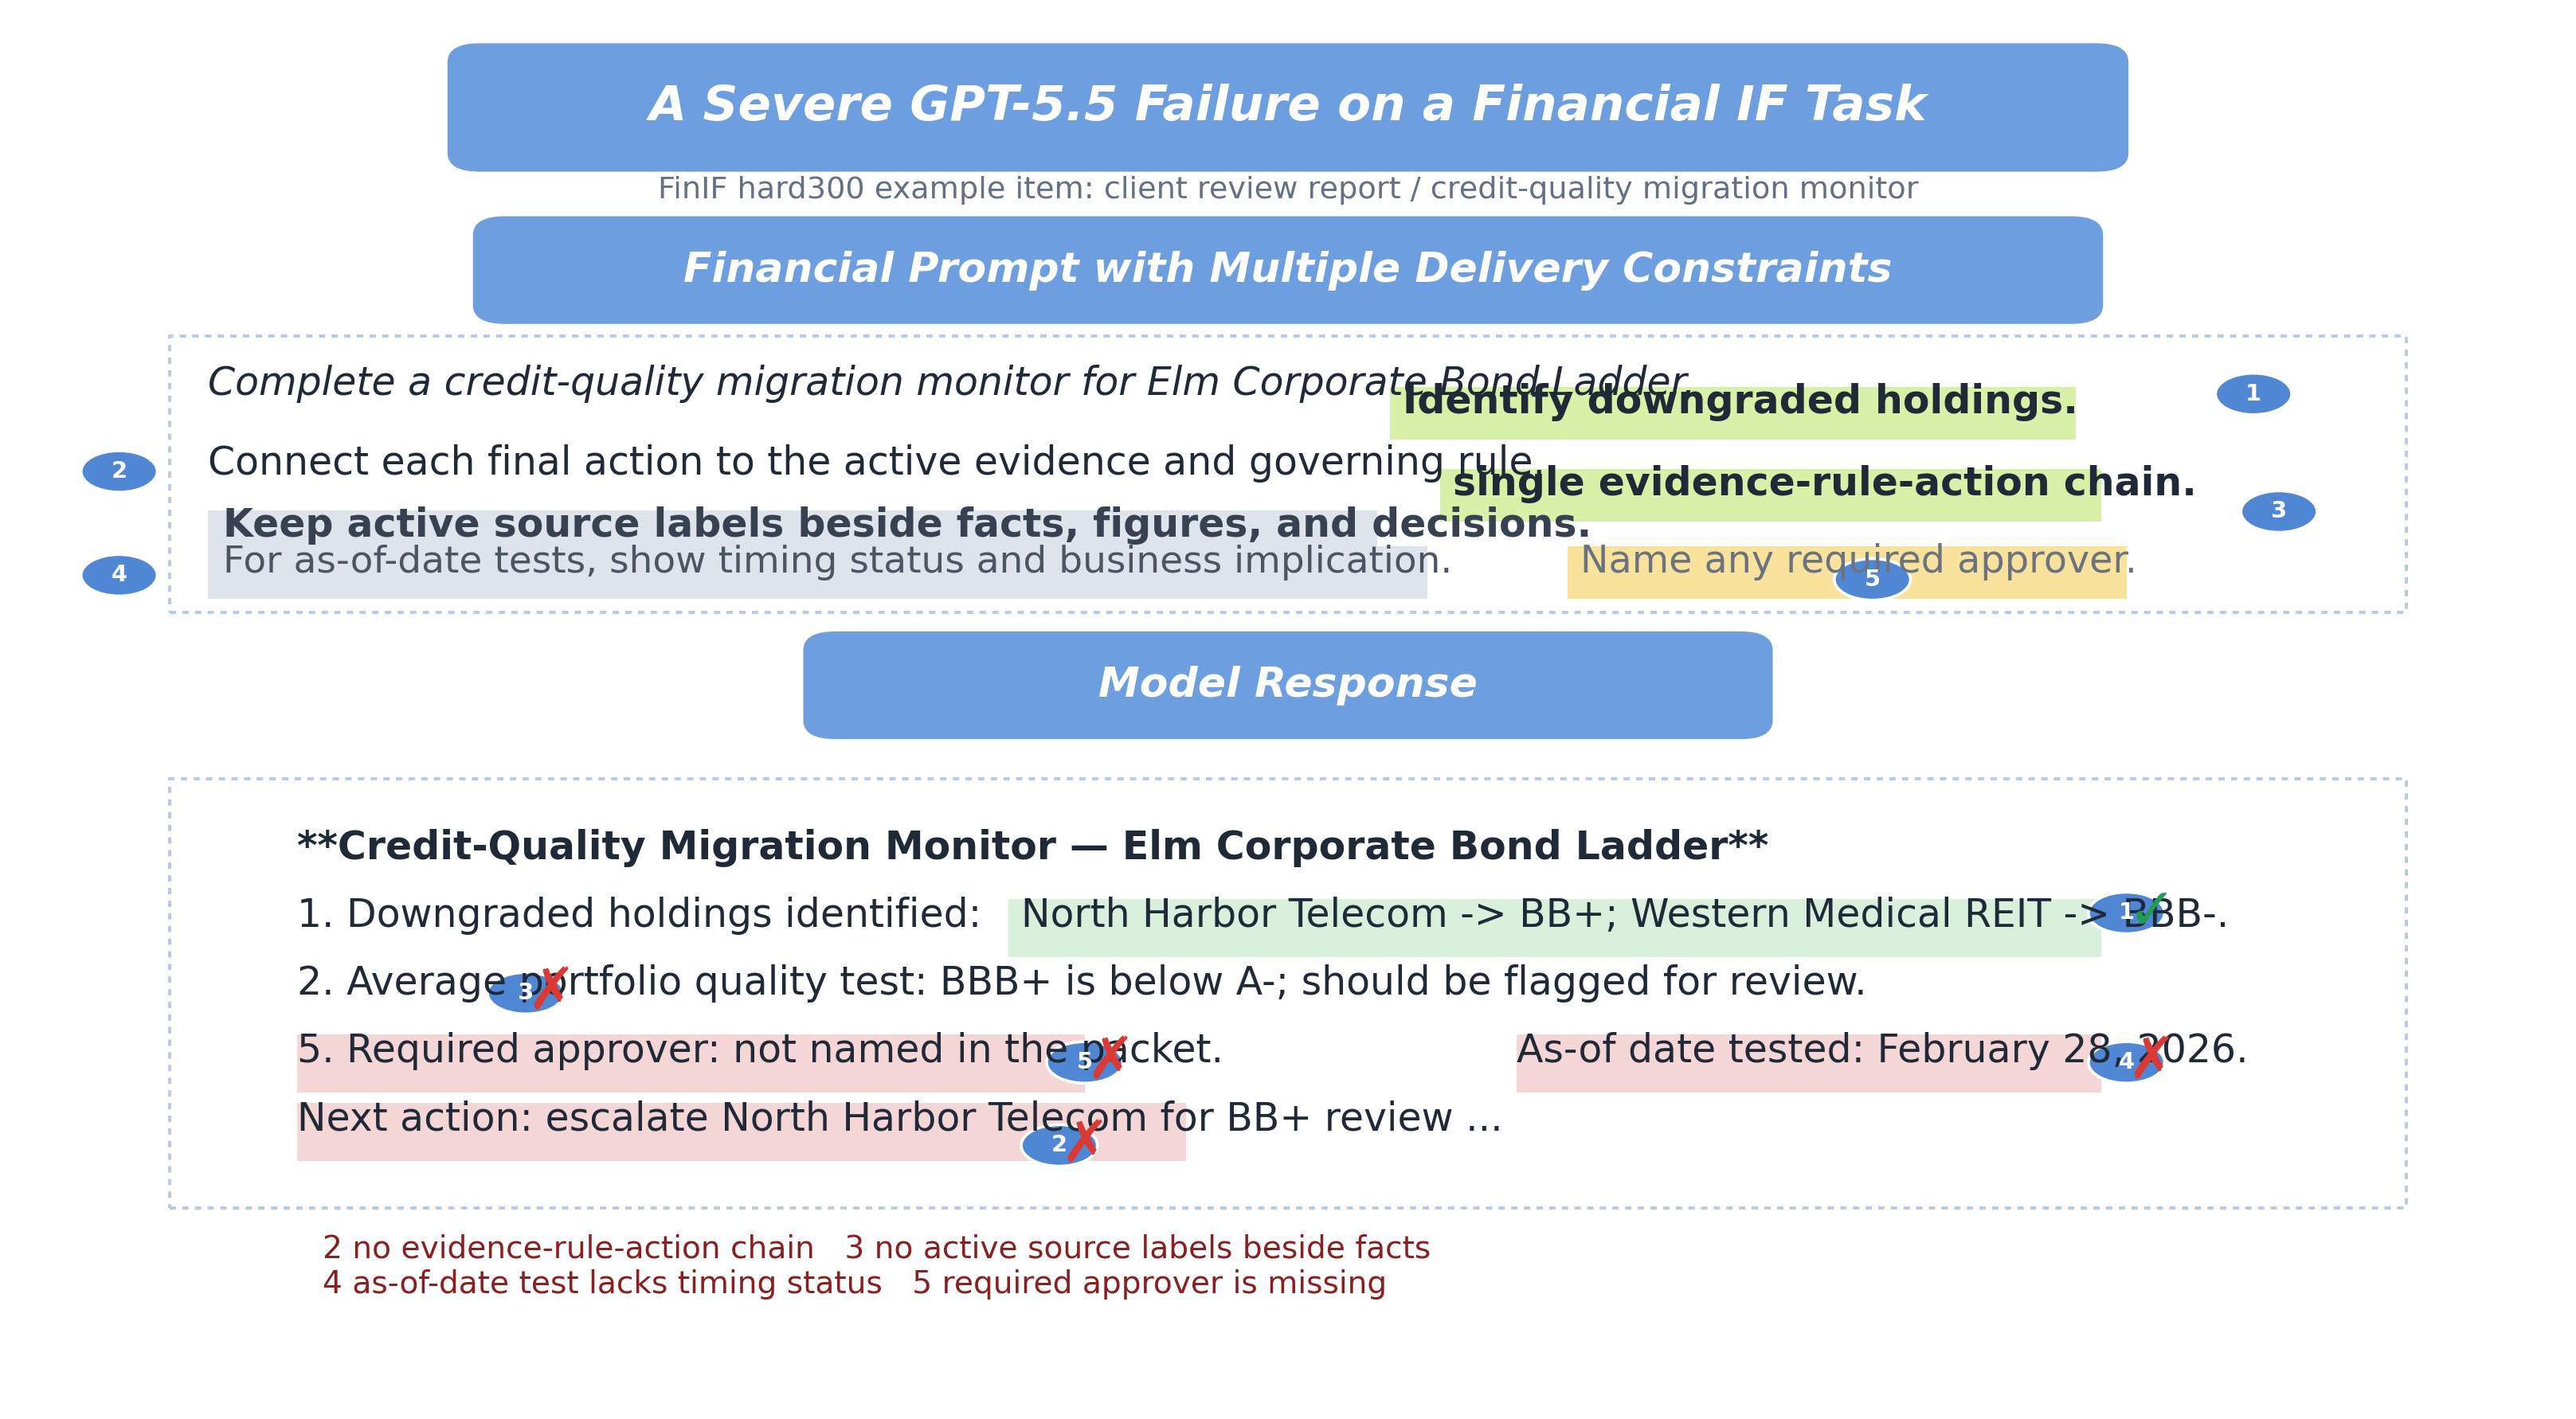
\includegraphics[width=\linewidth]{figures/figure1_finif_failures.png}
  \caption{A severe GPT-5.5 failure on a financial instruction-following task. The prompt asks for a credit-quality migration monitor with explicit delivery constraints. The model identifies the downgraded holdings, but still fails because it does not form a single evidence-rule-action chain, omits active source labels beside material facts, leaves the timing-status test incomplete, and does not name the required approver.}
  \label{fig:case}
\end{figure}

We present \textbf{FinIF}, a finance instruction-following benchmark suite. FinIF has two components. \textbf{FinIF-Test} is a 300-item hard benchmark selected from workflow-grounded finance tasks. It contains 3,134 instruction-following constraints, all evaluated with 100\% coverage in our experiments. \textbf{FinIF-Train} contains 1,064 workflow-grounded examples with 7,851 annotated constraints, intended for supervised training, preference-data construction, and further benchmark expansion.

FinIF differs from prior work in three ways. First, each item is built from a concrete financial workflow node and work product, rather than from a generic prompt template. Second, the benchmark separates instruction-following constraints from auxiliary diagnostic axes such as quality and finance validity. Third, the evaluator combines rule-based checking for mechanical constraints with LLM-as-a-judge scoring for semantic constraints, while reporting strict item-level compliance in addition to micro constraint pass rate.

Our experiments reveal that current models remain far from fully reliable on financial instruction following. GPT-5.5 passes 93.30\% of individual constraints but strictly passes only 58.67\% of items. GPT-5 passes 91.35\% of individual constraints but only 47.33\% of complete items. Smaller or cheaper models show a larger gap, with DS-V4-Pro, DS-V4-Flash, and Qwen3.5-9B reaching strict item pass rates of 16.00\%, 9.00\%, and 4.00\%, respectively. These results suggest that ``mostly compliant'' outputs are common, but complete compliant work products remain difficult.

Our contributions are:
\begin{itemize}
    \item We introduce FinIF-Test, a 300-item hard benchmark for evaluating instruction following in financial workflow tasks.
    \item We construct FinIF-Train, a 1,064-example workflow-grounded training pool with 7,851 annotated constraints.
    \item We propose a scalable construction pipeline and a dual-track evaluator that combines deterministic rule checks with item-batched LLM judging.
    \item We show that strong models still fail strict financial delivery requirements, especially evidence placement, quantitative verification, and decision-boundary reasoning.
\end{itemize}

\section{Related Work}

\subsection{Instruction Following of LLMs}

Instruction-following evaluation has become a central topic for LLM assessment. IFEval focuses on objectively verifiable instructions such as length, keyword, and format constraints, making evaluation reproducible and inexpensive \citep{zhou2023ifeval}. FollowBench broadens this line of work by testing fine-grained constraint following across multiple levels and constraint categories \citep{jiang2024followbench}. Other recent benchmarks further explore complex, real-user, or multi-constraint instruction following. These works demonstrate that instruction adherence should be evaluated separately from response quality. FinIF builds on this insight, but moves the evaluation target from general prompt constraints to finance-specific delivery requirements, including evidence discipline, quantitative lineage, and decision boundaries.

\subsection{Financial Capability Evaluation}

Financial LLM benchmarks usually focus on financial knowledge, numerical reasoning, information extraction, or business-domain task performance. FinEval evaluates financial domain knowledge and practical ability across academic, industry, security, and agent categories \citep{guo2023fineval}. CFinBench provides a large Chinese financial benchmark covering financial subjects, qualifications, practice, and law \citep{nie2024cfinbench}. BizFinBench emphasizes real-world financial applications and multi-dimensional financial task evaluation \citep{lu2025bizfinbench}. These benchmarks are valuable for measuring whether models know finance or can solve financial tasks. FinIF is complementary: it asks whether a model can obey the explicit delivery constraints that make a financial answer auditable, reviewable, and usable.

\section{Proposed Benchmark: FinIF}

FinIF is designed around financial work products. Each item provides context materials, a workflow-specific query, and explicit constraints extracted from the query or triggered by the context. The model must produce a financial deliverable, and the evaluator checks whether the response satisfies the requested instruction-following requirements.

\subsection{Task Taxonomy}

FinIF uses five workflow stages that cover a broad finance task lifecycle: Intake and Profiling; Research and Due Diligence; Decision and Structuring; Risk and Compliance Review; and Execution, Monitoring, Reporting, and Operations. These workflows are further decomposed into 38 task types. Examples include KYC onboarding, loan application intake, financial statement analysis, credit due diligence, investment memo drafting, DCF valuation, suitability review, AML red-flag review, reconciliation, board or regulatory reporting, and remediation tracking.

\begin{table}[t]
\centering
\small
\begin{tabular}{lrr}
\toprule
Workflow & Train items & Test items \\
\midrule
Intake and Profiling & 168 & 54 \\
Research and Due Diligence & 196 & 45 \\
Decision and Structuring & 224 & 63 \\
Risk and Compliance Review & 224 & 64 \\
Execution, Monitoring, Reporting, and Operations & 252 & 74 \\
\midrule
Total & 1,064 & 300 \\
\bottomrule
\end{tabular}
\caption{FinIF workflow coverage. FinIF-Train contains 1,064 workflow-grounded examples; FinIF-Test is a 300-item hard benchmark.}
\label{tab:workflow}
\end{table}

\subsection{Constraint Taxonomy}

FinIF evaluates explicit, checkable requirements rather than implicit best practices. We organize constraints into five families:
\begin{itemize}
    \item \textbf{Format and Presentation}: output structure, tables, exact labels, length, precision, opening and closing requirements.
    \item \textbf{Evidence and Grounding}: use of supplied context, citation placement, source fidelity, missing-data handling, and fact-inference separation.
    \item \textbf{Decision and Boundary}: decisions, escalation, approval, classification, regulated communication boundaries, and non-commitment requirements.
    \item \textbf{Quantitative Verification}: calculations, recalculation, reconciliation, thresholds, deadlines, ranking, and stress checks.
    \item \textbf{Required Content Coverage}: required deliverables, topics, issues, action items, profile factors, controls, and risk coverage.
\end{itemize}

\begin{table}[t]
\centering
\small
\begin{tabular}{lrrr}
\toprule
Constraint family & Train & Test IF & Test share \\
\midrule
Format and Presentation & 616 & 1,391 & 44.38\% \\
Evidence and Grounding & 1,990 & 1,085 & 34.62\% \\
Decision and Boundary & 1,885 & 280 & 8.93\% \\
Quantitative Verification & 1,456 & 377 & 12.03\% \\
Required Content Coverage & 1,904 & 1 & 0.03\% \\
\midrule
Total & 7,851 & 3,134 & 100.00\% \\
\bottomrule
\end{tabular}
\caption{Constraint distribution in FinIF-Train and FinIF-Test. FinIF-Test reports only instruction-following constraints; coverage, quality, and finance-validity diagnostics are kept separate.}
\label{tab:constraints}
\end{table}

\subsection{Data Construction}

The FinIF construction pipeline follows the sequence:
\[
\text{workflow} \rightarrow \text{task} \rightarrow \text{work product} \rightarrow \text{context} \rightarrow \text{query} \rightarrow \text{constraints} \rightarrow \text{evaluation protocol}.
\]

First, we sample a workflow and task type, then bind it to a specific financial work product, such as a KYC review note, credit memo, investment committee memo, suitability review note, compliance escalation report, reconciliation exception report, or board report. Next, we construct context packs from public primary sources, synthetic private records, or mixed packs. Public sources include regulatory guidance, SEC filings, FINRA materials, public financial statements, and similar primary materials. Private customer, borrower, account, and internal-policy records are synthetic to avoid exposing sensitive data.

We then write a natural workflow query that asks for the target work product. Explicit constraints are extracted from the query or from context-triggered requirements. Each constraint receives a fine-grained tag, a family label, an evaluation axis, and a checker route. We perform schema validation, query-diversity checks, and repair passes to reduce repetitive prompt skeletons and improve task coverage. The resulting 1,064 examples form FinIF-Train. FinIF-Test is selected as a hard 300-item subset with strong pressure on evidence, quantitative verification, decision boundaries, and explicit format requirements.

\subsection{Data Statistics}

FinIF-Train contains 1,064 items across all 38 task types, with 28 items per task and 7,851 annotated constraints. FinIF-Test contains 300 selected hard items, 3,134 instruction-following constraints, and 1,904 additional diagnostic constraints used for coverage, quality, and finance-validity analysis. The benchmark has an average of 10.45 IF constraints per item, with a minimum of 7 and a maximum of 16. Among IF constraints, 1,346 are rule-checked and 1,788 are LLM-judged.

\section{Capability Evaluation}

\subsection{Experimental Setup}

We evaluate five completed model runs on FinIF-Test: GPT-5.5, GPT-5, DS-V4-Pro, DS-V4-Flash, and Qwen3.5-9B. Each model is evaluated on the same 300-item hard benchmark containing 3,134 IF constraints. The evaluator reaches 100\% decision coverage for all reported full runs.

FinIF reports three main IF metrics. \textbf{Micro IF} is the fraction of passed constraints among all decided constraints. \textbf{Macro item IF} averages item-level constraint pass rates. \textbf{Strict item pass rate} counts an item as passed only if every IF constraint in that item is satisfied. We also report a holistic 0--10 quality score from the LLM judge as an auxiliary diagnostic, not as the primary IF metric.

The evaluator routes mechanically checkable constraints to deterministic rules, such as word ranges, decimal-place checks, required labels, table columns, first-line format, and ordered-list counts. Semantic constraints are batched by item and judged by GPT-4o with strict JSON parsing. This local-first design reduces judge calls while preserving coverage for constraints that require semantic judgment.

\subsection{Main Results}

\begin{table}[t]
\centering
\small
\begin{tabular}{lrrrr}
\toprule
Model & Micro IF & Macro IF & Strict pass & Quality \\
\midrule
GPT-5.5 & 93.30 & 93.10 & 58.67 & 7.40 \\
GPT-5 & 91.35 & 91.20 & 47.33 & 7.05 \\
DS-V4-Pro & 81.24 & 80.72 & 16.00 & 4.68 \\
DS-V4-Flash & 77.92 & 77.25 & 9.00 & 4.27 \\
Qwen3.5-9B & 72.08 & 71.45 & 4.00 & 3.60 \\
\bottomrule
\end{tabular}
\caption{Main results on FinIF-Test. IF metrics are percentages. Quality is a 0--10 auxiliary judge score. Strict pass requires satisfying every IF constraint in an item.}
\label{tab:main}
\end{table}

Table~\ref{tab:main} shows a large gap between constraint-level compliance and complete work-product compliance. GPT-5.5 passes 2,924 of 3,134 IF constraints, but strictly passes only 176 of 300 items. GPT-5 passes 2,863 constraints but strictly passes only 142 items. The gap is larger for cheaper and smaller models: DS-V4-Pro strictly passes 48 items, DS-V4-Flash 27 items, and Qwen3.5-9B only 12 items.

This result suggests that financial instruction following is best measured at multiple granularities. Micro IF captures whether a model follows many local requirements, while strict item pass rate captures whether the response is usable as a complete financial work product. In production-like settings, a response that violates one critical evidence or boundary instruction may still require human repair even if most local constraints pass.

\subsection{Further Analysis}

\paragraph{Evidence placement is the dominant failure mode.}
Across the evaluated models, the most frequent failed tag is EG2, which requires active source labels next to material facts, figures, thresholds, missing-evidence triggers, and decision points. GPT-5 fails 119 EG2 constraints, and GPT-5.5 fails 107. This indicates that even strong models often cite sources globally but fail to place evidence exactly where an audit trail requires it.

\paragraph{Quantitative verification remains fragile.}
The second recurring weakness is QV2, which requires source inputs, formula or comparison, result, and business implication for calculations and reconciliations. GPT-5 fails 42 QV2 constraints, while DS-V4-Pro and Qwen3.5-9B fail 113 and 162, respectively. These failures are not necessarily arithmetic mistakes; many are lineage failures where the response gives a number without the required verification trail.

\paragraph{Decision-boundary reasoning is hard to keep connected.}
DB9 asks the response to connect active evidence, governing rule or task standard, and final action in a single reasoning chain. GPT-5.5 and GPT-5 still fail 27 and 22 DB9 constraints, respectively. Smaller models fail this tag much more often. This suggests that models can list facts and recommendations, but often struggle to maintain an auditable evidence-rule-action chain.

\paragraph{Format constraints are not solved.}
Although many format checks are mechanically simple, they continue to cause item failures. GPT-5.5 fails 19 FP3 constraints, and GPT-5 fails 58. These include length, decimal-place, count, and ordering requirements. The Figure~\ref{fig:case} example shows why this matters: an otherwise high-quality response can be rejected because it fails a concrete delivery constraint.

\section{FinIF-Train}

FinIF-Train is the training and expansion component of FinIF. It contains 1,064 workflow-grounded examples, 38 task types, and 7,851 annotated constraints. Unlike generic instruction-tuning data, each example is tied to a finance workflow, a work product, and explicit delivery constraints. The goal is to support supervised fine-tuning or preference-data construction for finance instruction following.

The current repository contains the FinIF-Train data construction pipeline and the full 1,064-example pool. Full supervised fine-tuning results on the new FinIF-Test split are still ongoing and should not be conflated with earlier pilot results on the legacy 100-case benchmark. In the final submission, this section should be updated with same-split SFT results, ideally comparing a base model and a FinIF-trained model on the 300-item benchmark.

\todo{Add new-version SFT setup and results once Qwen/base and Qwen-SFT are scored on the same FinIF-Test hard300 split. Do not reuse the old 100-case SFT table as the main result.}

\section{Conclusion}

We introduced FinIF, a finance instruction-following benchmark suite for evaluating whether LLMs can produce usable financial work products under explicit delivery constraints. FinIF-Test provides a 300-item hard benchmark with 3,134 IF constraints, while FinIF-Train provides 1,064 workflow-grounded examples for training and expansion. Experiments show that strong models satisfy most individual constraints but frequently fail strict item-level compliance. The largest weaknesses involve evidence placement, quantitative verification, and decision-boundary reasoning. These findings suggest that financial LLM evaluation should measure not only answer quality, but also whether the answer follows the operational instructions needed for auditability and downstream use.

\section{Limitations}

FinIF has several limitations. First, semantic evaluation depends on an LLM judge, so additional human calibration and judge-sensitivity analysis are needed. Second, some private financial records are synthetic, which improves privacy and control but may not capture all real institution-specific variation. Third, the current reported experiments cover five completed model runs; additional open-weight, finance-tuned, and newly trained FinIF models should be added. Fourth, FinIF-Test emphasizes hard instruction-following cases, so its strict pass rates should not be interpreted as general financial task success rates. Finally, supervised training results for the new 300-item split are not yet included in this draft.

\begin{thebibliography}{}

\bibitem[Zhou et~al.(2023)]{zhou2023ifeval}
Jeffrey Zhou, Tianjian Lu, Swaroop Mishra, Siddhartha Brahma, Sujoy Basu, Yi Luan, Denny Zhou, and Le Hou. 2023.
\newblock Instruction-Following Evaluation for Large Language Models.
\newblock \emph{arXiv:2311.07911}.

\bibitem[Jiang et~al.(2024)]{jiang2024followbench}
Yuxin Jiang, Yufei Wang, Xingshan Zeng, Wanjun Zhong, Liangyou Li, Fei Mi, Lifeng Shang, Xin Jiang, Qun Liu, and Wei Wang. 2024.
\newblock FollowBench: A Multi-level Fine-grained Constraints Following Benchmark for Large Language Models.
\newblock \emph{ACL 2024}.

\bibitem[Guo et~al.(2023)]{guo2023fineval}
Xin Guo, Haotian Xia, Zhaowei Liu, Hanyang Cao, Zhi Yang, Zhiqiang Liu, Sizhe Wang, Jinyi Niu, Chuqi Wang, Yanhui Wang, Xiaolong Liang, Xiaoming Huang, Bing Zhu, Zhongyu Wei, Yun Chen, Weining Shen, and Liwen Zhang. 2023.
\newblock FinEval: A Chinese Financial Domain Knowledge Evaluation Benchmark for Large Language Models.
\newblock \emph{arXiv:2308.09975}.

\bibitem[Nie et~al.(2024)]{nie2024cfinbench}
Ying Nie, Binwei Yan, Tianyu Guo, Hao Liu, Haoyu Wang, Wei He, Binfan Zheng, Weihao Wang, Qiang Li, Weijian Sun, Yunhe Wang, and Dacheng Tao. 2024.
\newblock CFinBench: A Comprehensive Chinese Financial Benchmark for Large Language Models.
\newblock \emph{arXiv:2407.02301}.

\bibitem[Lu et~al.(2025)]{lu2025bizfinbench}
Guilong Lu, Xuntao Guo, Rongjunchen Zhang, Wenqiao Zhu, and Ji Liu. 2025.
\newblock BizFinBench: A Business-Driven Real-World Financial Benchmark for Evaluating LLMs.
\newblock \emph{arXiv:2505.19457}.

\end{thebibliography}

\end{document}
